\documentclass[11pt]{article}

    \usepackage[breakable]{tcolorbox}
    \usepackage{parskip} % Stop auto-indenting (to mimic markdown behaviour)
    
    \usepackage{iftex}
    \ifPDFTeX
    	\usepackage[T1]{fontenc}
    	\usepackage{mathpazo}
    \else
    	\usepackage{fontspec}
    \fi

    % Basic figure setup, for now with no caption control since it's done
    % automatically by Pandoc (which extracts ![](path) syntax from Markdown).
    \usepackage{graphicx}
    % Maintain compatibility with old templates. Remove in nbconvert 6.0
    \let\Oldincludegraphics\includegraphics
    % Ensure that by default, figures have no caption (until we provide a
    % proper Figure object with a Caption API and a way to capture that
    % in the conversion process - todo).
    \usepackage{caption}
    \DeclareCaptionFormat{nocaption}{}
    \captionsetup{format=nocaption,aboveskip=0pt,belowskip=0pt}

    \usepackage[Export]{adjustbox} % Used to constrain images to a maximum size
    \adjustboxset{max size={0.9\linewidth}{0.9\paperheight}}
    \usepackage{float}
    \floatplacement{figure}{H} % forces figures to be placed at the correct location
    \usepackage{xcolor} % Allow colors to be defined
    \usepackage{enumerate} % Needed for markdown enumerations to work
    \usepackage{geometry} % Used to adjust the document margins
    \usepackage{amsmath} % Equations
    \usepackage{amssymb} % Equations
    \usepackage{textcomp} % defines textquotesingle
    % Hack from http://tex.stackexchange.com/a/47451/13684:
    \AtBeginDocument{%
        \def\PYZsq{\textquotesingle}% Upright quotes in Pygmentized code
    }
    \usepackage{upquote} % Upright quotes for verbatim code
    \usepackage{eurosym} % defines \euro
    \usepackage[mathletters]{ucs} % Extended unicode (utf-8) support
    \usepackage{fancyvrb} % verbatim replacement that allows latex

    % The hyperref package gives us a pdf with properly built
    % internal navigation ('pdf bookmarks' for the table of contents,
    % internal cross-reference links, web links for URLs, etc.)
    \usepackage{hyperref}
    % The default LaTeX title has an obnoxious amount of whitespace. By default,
    % titling removes some of it. It also provides customization options.
    \usepackage{titling}
    \usepackage{longtable} % longtable support required by pandoc >1.10
    \usepackage{booktabs}  % table support for pandoc > 1.12.2
    \usepackage[inline]{enumitem} % IRkernel/repr support (it uses the enumerate* environment)
    \usepackage[normalem]{ulem} % ulem is needed to support strikethroughs (\sout)
                                % normalem makes italics be italics, not underlines
    \usepackage{mathrsfs}
    

    
    % Colors for the hyperref package
    \definecolor{urlcolor}{rgb}{0,.145,.698}
    \definecolor{linkcolor}{rgb}{.71,0.21,0.01}
    \definecolor{citecolor}{rgb}{.12,.54,.11}

    % ANSI colors
    \definecolor{ansi-black}{HTML}{3E424D}
    \definecolor{ansi-black-intense}{HTML}{282C36}
    \definecolor{ansi-red}{HTML}{E75C58}
    \definecolor{ansi-red-intense}{HTML}{B22B31}
    \definecolor{ansi-green}{HTML}{00A250}
    \definecolor{ansi-green-intense}{HTML}{007427}
    \definecolor{ansi-yellow}{HTML}{DDB62B}
    \definecolor{ansi-yellow-intense}{HTML}{B27D12}
    \definecolor{ansi-blue}{HTML}{208FFB}
    \definecolor{ansi-blue-intense}{HTML}{0065CA}
    \definecolor{ansi-magenta}{HTML}{D160C4}
    \definecolor{ansi-magenta-intense}{HTML}{A03196}
    \definecolor{ansi-cyan}{HTML}{60C6C8}
    \definecolor{ansi-cyan-intense}{HTML}{258F8F}
    \definecolor{ansi-white}{HTML}{C5C1B4}
    \definecolor{ansi-white-intense}{HTML}{A1A6B2}
    \definecolor{ansi-default-inverse-fg}{HTML}{FFFFFF}
    \definecolor{ansi-default-inverse-bg}{HTML}{000000}

    % commands and environments needed by pandoc snippets
    % extracted from the output of `pandoc -s`
    \providecommand{\tightlist}{%
      \setlength{\itemsep}{0pt}\setlength{\parskip}{0pt}}
    \DefineVerbatimEnvironment{Highlighting}{Verbatim}{commandchars=\\\{\}}
    % Add ',fontsize=\small' for more characters per line
    \newenvironment{Shaded}{}{}
    \newcommand{\KeywordTok}[1]{\textcolor[rgb]{0.00,0.44,0.13}{\textbf{{#1}}}}
    \newcommand{\DataTypeTok}[1]{\textcolor[rgb]{0.56,0.13,0.00}{{#1}}}
    \newcommand{\DecValTok}[1]{\textcolor[rgb]{0.25,0.63,0.44}{{#1}}}
    \newcommand{\BaseNTok}[1]{\textcolor[rgb]{0.25,0.63,0.44}{{#1}}}
    \newcommand{\FloatTok}[1]{\textcolor[rgb]{0.25,0.63,0.44}{{#1}}}
    \newcommand{\CharTok}[1]{\textcolor[rgb]{0.25,0.44,0.63}{{#1}}}
    \newcommand{\StringTok}[1]{\textcolor[rgb]{0.25,0.44,0.63}{{#1}}}
    \newcommand{\CommentTok}[1]{\textcolor[rgb]{0.38,0.63,0.69}{\textit{{#1}}}}
    \newcommand{\OtherTok}[1]{\textcolor[rgb]{0.00,0.44,0.13}{{#1}}}
    \newcommand{\AlertTok}[1]{\textcolor[rgb]{1.00,0.00,0.00}{\textbf{{#1}}}}
    \newcommand{\FunctionTok}[1]{\textcolor[rgb]{0.02,0.16,0.49}{{#1}}}
    \newcommand{\RegionMarkerTok}[1]{{#1}}
    \newcommand{\ErrorTok}[1]{\textcolor[rgb]{1.00,0.00,0.00}{\textbf{{#1}}}}
    \newcommand{\NormalTok}[1]{{#1}}
    
    % Additional commands for more recent versions of Pandoc
    \newcommand{\ConstantTok}[1]{\textcolor[rgb]{0.53,0.00,0.00}{{#1}}}
    \newcommand{\SpecialCharTok}[1]{\textcolor[rgb]{0.25,0.44,0.63}{{#1}}}
    \newcommand{\VerbatimStringTok}[1]{\textcolor[rgb]{0.25,0.44,0.63}{{#1}}}
    \newcommand{\SpecialStringTok}[1]{\textcolor[rgb]{0.73,0.40,0.53}{{#1}}}
    \newcommand{\ImportTok}[1]{{#1}}
    \newcommand{\DocumentationTok}[1]{\textcolor[rgb]{0.73,0.13,0.13}{\textit{{#1}}}}
    \newcommand{\AnnotationTok}[1]{\textcolor[rgb]{0.38,0.63,0.69}{\textbf{\textit{{#1}}}}}
    \newcommand{\CommentVarTok}[1]{\textcolor[rgb]{0.38,0.63,0.69}{\textbf{\textit{{#1}}}}}
    \newcommand{\VariableTok}[1]{\textcolor[rgb]{0.10,0.09,0.49}{{#1}}}
    \newcommand{\ControlFlowTok}[1]{\textcolor[rgb]{0.00,0.44,0.13}{\textbf{{#1}}}}
    \newcommand{\OperatorTok}[1]{\textcolor[rgb]{0.40,0.40,0.40}{{#1}}}
    \newcommand{\BuiltInTok}[1]{{#1}}
    \newcommand{\ExtensionTok}[1]{{#1}}
    \newcommand{\PreprocessorTok}[1]{\textcolor[rgb]{0.74,0.48,0.00}{{#1}}}
    \newcommand{\AttributeTok}[1]{\textcolor[rgb]{0.49,0.56,0.16}{{#1}}}
    \newcommand{\InformationTok}[1]{\textcolor[rgb]{0.38,0.63,0.69}{\textbf{\textit{{#1}}}}}
    \newcommand{\WarningTok}[1]{\textcolor[rgb]{0.38,0.63,0.69}{\textbf{\textit{{#1}}}}}
    
    
    % Define a nice break command that doesn't care if a line doesn't already
    % exist.
    \def\br{\hspace*{\fill} \\* }
    % Math Jax compatibility definitions
    \def\gt{>}
    \def\lt{<}
    \let\Oldtex\TeX
    \let\Oldlatex\LaTeX
    \renewcommand{\TeX}{\textrm{\Oldtex}}
    \renewcommand{\LaTeX}{\textrm{\Oldlatex}}
    % Document parameters
    % Document title
    \title{OOP}
    
    
    
    
    
% Pygments definitions
\makeatletter
\def\PY@reset{\let\PY@it=\relax \let\PY@bf=\relax%
    \let\PY@ul=\relax \let\PY@tc=\relax%
    \let\PY@bc=\relax \let\PY@ff=\relax}
\def\PY@tok#1{\csname PY@tok@#1\endcsname}
\def\PY@toks#1+{\ifx\relax#1\empty\else%
    \PY@tok{#1}\expandafter\PY@toks\fi}
\def\PY@do#1{\PY@bc{\PY@tc{\PY@ul{%
    \PY@it{\PY@bf{\PY@ff{#1}}}}}}}
\def\PY#1#2{\PY@reset\PY@toks#1+\relax+\PY@do{#2}}

\expandafter\def\csname PY@tok@w\endcsname{\def\PY@tc##1{\textcolor[rgb]{0.73,0.73,0.73}{##1}}}
\expandafter\def\csname PY@tok@c\endcsname{\let\PY@it=\textit\def\PY@tc##1{\textcolor[rgb]{0.25,0.50,0.50}{##1}}}
\expandafter\def\csname PY@tok@cp\endcsname{\def\PY@tc##1{\textcolor[rgb]{0.74,0.48,0.00}{##1}}}
\expandafter\def\csname PY@tok@k\endcsname{\let\PY@bf=\textbf\def\PY@tc##1{\textcolor[rgb]{0.00,0.50,0.00}{##1}}}
\expandafter\def\csname PY@tok@kp\endcsname{\def\PY@tc##1{\textcolor[rgb]{0.00,0.50,0.00}{##1}}}
\expandafter\def\csname PY@tok@kt\endcsname{\def\PY@tc##1{\textcolor[rgb]{0.69,0.00,0.25}{##1}}}
\expandafter\def\csname PY@tok@o\endcsname{\def\PY@tc##1{\textcolor[rgb]{0.40,0.40,0.40}{##1}}}
\expandafter\def\csname PY@tok@ow\endcsname{\let\PY@bf=\textbf\def\PY@tc##1{\textcolor[rgb]{0.67,0.13,1.00}{##1}}}
\expandafter\def\csname PY@tok@nb\endcsname{\def\PY@tc##1{\textcolor[rgb]{0.00,0.50,0.00}{##1}}}
\expandafter\def\csname PY@tok@nf\endcsname{\def\PY@tc##1{\textcolor[rgb]{0.00,0.00,1.00}{##1}}}
\expandafter\def\csname PY@tok@nc\endcsname{\let\PY@bf=\textbf\def\PY@tc##1{\textcolor[rgb]{0.00,0.00,1.00}{##1}}}
\expandafter\def\csname PY@tok@nn\endcsname{\let\PY@bf=\textbf\def\PY@tc##1{\textcolor[rgb]{0.00,0.00,1.00}{##1}}}
\expandafter\def\csname PY@tok@ne\endcsname{\let\PY@bf=\textbf\def\PY@tc##1{\textcolor[rgb]{0.82,0.25,0.23}{##1}}}
\expandafter\def\csname PY@tok@nv\endcsname{\def\PY@tc##1{\textcolor[rgb]{0.10,0.09,0.49}{##1}}}
\expandafter\def\csname PY@tok@no\endcsname{\def\PY@tc##1{\textcolor[rgb]{0.53,0.00,0.00}{##1}}}
\expandafter\def\csname PY@tok@nl\endcsname{\def\PY@tc##1{\textcolor[rgb]{0.63,0.63,0.00}{##1}}}
\expandafter\def\csname PY@tok@ni\endcsname{\let\PY@bf=\textbf\def\PY@tc##1{\textcolor[rgb]{0.60,0.60,0.60}{##1}}}
\expandafter\def\csname PY@tok@na\endcsname{\def\PY@tc##1{\textcolor[rgb]{0.49,0.56,0.16}{##1}}}
\expandafter\def\csname PY@tok@nt\endcsname{\let\PY@bf=\textbf\def\PY@tc##1{\textcolor[rgb]{0.00,0.50,0.00}{##1}}}
\expandafter\def\csname PY@tok@nd\endcsname{\def\PY@tc##1{\textcolor[rgb]{0.67,0.13,1.00}{##1}}}
\expandafter\def\csname PY@tok@s\endcsname{\def\PY@tc##1{\textcolor[rgb]{0.73,0.13,0.13}{##1}}}
\expandafter\def\csname PY@tok@sd\endcsname{\let\PY@it=\textit\def\PY@tc##1{\textcolor[rgb]{0.73,0.13,0.13}{##1}}}
\expandafter\def\csname PY@tok@si\endcsname{\let\PY@bf=\textbf\def\PY@tc##1{\textcolor[rgb]{0.73,0.40,0.53}{##1}}}
\expandafter\def\csname PY@tok@se\endcsname{\let\PY@bf=\textbf\def\PY@tc##1{\textcolor[rgb]{0.73,0.40,0.13}{##1}}}
\expandafter\def\csname PY@tok@sr\endcsname{\def\PY@tc##1{\textcolor[rgb]{0.73,0.40,0.53}{##1}}}
\expandafter\def\csname PY@tok@ss\endcsname{\def\PY@tc##1{\textcolor[rgb]{0.10,0.09,0.49}{##1}}}
\expandafter\def\csname PY@tok@sx\endcsname{\def\PY@tc##1{\textcolor[rgb]{0.00,0.50,0.00}{##1}}}
\expandafter\def\csname PY@tok@m\endcsname{\def\PY@tc##1{\textcolor[rgb]{0.40,0.40,0.40}{##1}}}
\expandafter\def\csname PY@tok@gh\endcsname{\let\PY@bf=\textbf\def\PY@tc##1{\textcolor[rgb]{0.00,0.00,0.50}{##1}}}
\expandafter\def\csname PY@tok@gu\endcsname{\let\PY@bf=\textbf\def\PY@tc##1{\textcolor[rgb]{0.50,0.00,0.50}{##1}}}
\expandafter\def\csname PY@tok@gd\endcsname{\def\PY@tc##1{\textcolor[rgb]{0.63,0.00,0.00}{##1}}}
\expandafter\def\csname PY@tok@gi\endcsname{\def\PY@tc##1{\textcolor[rgb]{0.00,0.63,0.00}{##1}}}
\expandafter\def\csname PY@tok@gr\endcsname{\def\PY@tc##1{\textcolor[rgb]{1.00,0.00,0.00}{##1}}}
\expandafter\def\csname PY@tok@ge\endcsname{\let\PY@it=\textit}
\expandafter\def\csname PY@tok@gs\endcsname{\let\PY@bf=\textbf}
\expandafter\def\csname PY@tok@gp\endcsname{\let\PY@bf=\textbf\def\PY@tc##1{\textcolor[rgb]{0.00,0.00,0.50}{##1}}}
\expandafter\def\csname PY@tok@go\endcsname{\def\PY@tc##1{\textcolor[rgb]{0.53,0.53,0.53}{##1}}}
\expandafter\def\csname PY@tok@gt\endcsname{\def\PY@tc##1{\textcolor[rgb]{0.00,0.27,0.87}{##1}}}
\expandafter\def\csname PY@tok@err\endcsname{\def\PY@bc##1{\setlength{\fboxsep}{0pt}\fcolorbox[rgb]{1.00,0.00,0.00}{1,1,1}{\strut ##1}}}
\expandafter\def\csname PY@tok@kc\endcsname{\let\PY@bf=\textbf\def\PY@tc##1{\textcolor[rgb]{0.00,0.50,0.00}{##1}}}
\expandafter\def\csname PY@tok@kd\endcsname{\let\PY@bf=\textbf\def\PY@tc##1{\textcolor[rgb]{0.00,0.50,0.00}{##1}}}
\expandafter\def\csname PY@tok@kn\endcsname{\let\PY@bf=\textbf\def\PY@tc##1{\textcolor[rgb]{0.00,0.50,0.00}{##1}}}
\expandafter\def\csname PY@tok@kr\endcsname{\let\PY@bf=\textbf\def\PY@tc##1{\textcolor[rgb]{0.00,0.50,0.00}{##1}}}
\expandafter\def\csname PY@tok@bp\endcsname{\def\PY@tc##1{\textcolor[rgb]{0.00,0.50,0.00}{##1}}}
\expandafter\def\csname PY@tok@fm\endcsname{\def\PY@tc##1{\textcolor[rgb]{0.00,0.00,1.00}{##1}}}
\expandafter\def\csname PY@tok@vc\endcsname{\def\PY@tc##1{\textcolor[rgb]{0.10,0.09,0.49}{##1}}}
\expandafter\def\csname PY@tok@vg\endcsname{\def\PY@tc##1{\textcolor[rgb]{0.10,0.09,0.49}{##1}}}
\expandafter\def\csname PY@tok@vi\endcsname{\def\PY@tc##1{\textcolor[rgb]{0.10,0.09,0.49}{##1}}}
\expandafter\def\csname PY@tok@vm\endcsname{\def\PY@tc##1{\textcolor[rgb]{0.10,0.09,0.49}{##1}}}
\expandafter\def\csname PY@tok@sa\endcsname{\def\PY@tc##1{\textcolor[rgb]{0.73,0.13,0.13}{##1}}}
\expandafter\def\csname PY@tok@sb\endcsname{\def\PY@tc##1{\textcolor[rgb]{0.73,0.13,0.13}{##1}}}
\expandafter\def\csname PY@tok@sc\endcsname{\def\PY@tc##1{\textcolor[rgb]{0.73,0.13,0.13}{##1}}}
\expandafter\def\csname PY@tok@dl\endcsname{\def\PY@tc##1{\textcolor[rgb]{0.73,0.13,0.13}{##1}}}
\expandafter\def\csname PY@tok@s2\endcsname{\def\PY@tc##1{\textcolor[rgb]{0.73,0.13,0.13}{##1}}}
\expandafter\def\csname PY@tok@sh\endcsname{\def\PY@tc##1{\textcolor[rgb]{0.73,0.13,0.13}{##1}}}
\expandafter\def\csname PY@tok@s1\endcsname{\def\PY@tc##1{\textcolor[rgb]{0.73,0.13,0.13}{##1}}}
\expandafter\def\csname PY@tok@mb\endcsname{\def\PY@tc##1{\textcolor[rgb]{0.40,0.40,0.40}{##1}}}
\expandafter\def\csname PY@tok@mf\endcsname{\def\PY@tc##1{\textcolor[rgb]{0.40,0.40,0.40}{##1}}}
\expandafter\def\csname PY@tok@mh\endcsname{\def\PY@tc##1{\textcolor[rgb]{0.40,0.40,0.40}{##1}}}
\expandafter\def\csname PY@tok@mi\endcsname{\def\PY@tc##1{\textcolor[rgb]{0.40,0.40,0.40}{##1}}}
\expandafter\def\csname PY@tok@il\endcsname{\def\PY@tc##1{\textcolor[rgb]{0.40,0.40,0.40}{##1}}}
\expandafter\def\csname PY@tok@mo\endcsname{\def\PY@tc##1{\textcolor[rgb]{0.40,0.40,0.40}{##1}}}
\expandafter\def\csname PY@tok@ch\endcsname{\let\PY@it=\textit\def\PY@tc##1{\textcolor[rgb]{0.25,0.50,0.50}{##1}}}
\expandafter\def\csname PY@tok@cm\endcsname{\let\PY@it=\textit\def\PY@tc##1{\textcolor[rgb]{0.25,0.50,0.50}{##1}}}
\expandafter\def\csname PY@tok@cpf\endcsname{\let\PY@it=\textit\def\PY@tc##1{\textcolor[rgb]{0.25,0.50,0.50}{##1}}}
\expandafter\def\csname PY@tok@c1\endcsname{\let\PY@it=\textit\def\PY@tc##1{\textcolor[rgb]{0.25,0.50,0.50}{##1}}}
\expandafter\def\csname PY@tok@cs\endcsname{\let\PY@it=\textit\def\PY@tc##1{\textcolor[rgb]{0.25,0.50,0.50}{##1}}}

\def\PYZbs{\char`\\}
\def\PYZus{\char`\_}
\def\PYZob{\char`\{}
\def\PYZcb{\char`\}}
\def\PYZca{\char`\^}
\def\PYZam{\char`\&}
\def\PYZlt{\char`\<}
\def\PYZgt{\char`\>}
\def\PYZsh{\char`\#}
\def\PYZpc{\char`\%}
\def\PYZdl{\char`\$}
\def\PYZhy{\char`\-}
\def\PYZsq{\char`\'}
\def\PYZdq{\char`\"}
\def\PYZti{\char`\~}
% for compatibility with earlier versions
\def\PYZat{@}
\def\PYZlb{[}
\def\PYZrb{]}
\makeatother


    % For linebreaks inside Verbatim environment from package fancyvrb. 
    \makeatletter
        \newbox\Wrappedcontinuationbox 
        \newbox\Wrappedvisiblespacebox 
        \newcommand*\Wrappedvisiblespace {\textcolor{red}{\textvisiblespace}} 
        \newcommand*\Wrappedcontinuationsymbol {\textcolor{red}{\llap{\tiny$\m@th\hookrightarrow$}}} 
        \newcommand*\Wrappedcontinuationindent {3ex } 
        \newcommand*\Wrappedafterbreak {\kern\Wrappedcontinuationindent\copy\Wrappedcontinuationbox} 
        % Take advantage of the already applied Pygments mark-up to insert 
        % potential linebreaks for TeX processing. 
        %        {, <, #, %, $, ' and ": go to next line. 
        %        _, }, ^, &, >, - and ~: stay at end of broken line. 
        % Use of \textquotesingle for straight quote. 
        \newcommand*\Wrappedbreaksatspecials {% 
            \def\PYGZus{\discretionary{\char`\_}{\Wrappedafterbreak}{\char`\_}}% 
            \def\PYGZob{\discretionary{}{\Wrappedafterbreak\char`\{}{\char`\{}}% 
            \def\PYGZcb{\discretionary{\char`\}}{\Wrappedafterbreak}{\char`\}}}% 
            \def\PYGZca{\discretionary{\char`\^}{\Wrappedafterbreak}{\char`\^}}% 
            \def\PYGZam{\discretionary{\char`\&}{\Wrappedafterbreak}{\char`\&}}% 
            \def\PYGZlt{\discretionary{}{\Wrappedafterbreak\char`\<}{\char`\<}}% 
            \def\PYGZgt{\discretionary{\char`\>}{\Wrappedafterbreak}{\char`\>}}% 
            \def\PYGZsh{\discretionary{}{\Wrappedafterbreak\char`\#}{\char`\#}}% 
            \def\PYGZpc{\discretionary{}{\Wrappedafterbreak\char`\%}{\char`\%}}% 
            \def\PYGZdl{\discretionary{}{\Wrappedafterbreak\char`\$}{\char`\$}}% 
            \def\PYGZhy{\discretionary{\char`\-}{\Wrappedafterbreak}{\char`\-}}% 
            \def\PYGZsq{\discretionary{}{\Wrappedafterbreak\textquotesingle}{\textquotesingle}}% 
            \def\PYGZdq{\discretionary{}{\Wrappedafterbreak\char`\"}{\char`\"}}% 
            \def\PYGZti{\discretionary{\char`\~}{\Wrappedafterbreak}{\char`\~}}% 
        } 
        % Some characters . , ; ? ! / are not pygmentized. 
        % This macro makes them "active" and they will insert potential linebreaks 
        \newcommand*\Wrappedbreaksatpunct {% 
            \lccode`\~`\.\lowercase{\def~}{\discretionary{\hbox{\char`\.}}{\Wrappedafterbreak}{\hbox{\char`\.}}}% 
            \lccode`\~`\,\lowercase{\def~}{\discretionary{\hbox{\char`\,}}{\Wrappedafterbreak}{\hbox{\char`\,}}}% 
            \lccode`\~`\;\lowercase{\def~}{\discretionary{\hbox{\char`\;}}{\Wrappedafterbreak}{\hbox{\char`\;}}}% 
            \lccode`\~`\:\lowercase{\def~}{\discretionary{\hbox{\char`\:}}{\Wrappedafterbreak}{\hbox{\char`\:}}}% 
            \lccode`\~`\?\lowercase{\def~}{\discretionary{\hbox{\char`\?}}{\Wrappedafterbreak}{\hbox{\char`\?}}}% 
            \lccode`\~`\!\lowercase{\def~}{\discretionary{\hbox{\char`\!}}{\Wrappedafterbreak}{\hbox{\char`\!}}}% 
            \lccode`\~`\/\lowercase{\def~}{\discretionary{\hbox{\char`\/}}{\Wrappedafterbreak}{\hbox{\char`\/}}}% 
            \catcode`\.\active
            \catcode`\,\active 
            \catcode`\;\active
            \catcode`\:\active
            \catcode`\?\active
            \catcode`\!\active
            \catcode`\/\active 
            \lccode`\~`\~ 	
        }
    \makeatother

    \let\OriginalVerbatim=\Verbatim
    \makeatletter
    \renewcommand{\Verbatim}[1][1]{%
        %\parskip\z@skip
        \sbox\Wrappedcontinuationbox {\Wrappedcontinuationsymbol}%
        \sbox\Wrappedvisiblespacebox {\FV@SetupFont\Wrappedvisiblespace}%
        \def\FancyVerbFormatLine ##1{\hsize\linewidth
            \vtop{\raggedright\hyphenpenalty\z@\exhyphenpenalty\z@
                \doublehyphendemerits\z@\finalhyphendemerits\z@
                \strut ##1\strut}%
        }%
        % If the linebreak is at a space, the latter will be displayed as visible
        % space at end of first line, and a continuation symbol starts next line.
        % Stretch/shrink are however usually zero for typewriter font.
        \def\FV@Space {%
            \nobreak\hskip\z@ plus\fontdimen3\font minus\fontdimen4\font
            \discretionary{\copy\Wrappedvisiblespacebox}{\Wrappedafterbreak}
            {\kern\fontdimen2\font}%
        }%
        
        % Allow breaks at special characters using \PYG... macros.
        \Wrappedbreaksatspecials
        % Breaks at punctuation characters . , ; ? ! and / need catcode=\active 	
        \OriginalVerbatim[#1,codes*=\Wrappedbreaksatpunct]%
    }
    \makeatother

    % Exact colors from NB
    \definecolor{incolor}{HTML}{303F9F}
    \definecolor{outcolor}{HTML}{D84315}
    \definecolor{cellborder}{HTML}{CFCFCF}
    \definecolor{cellbackground}{HTML}{F7F7F7}
    
    % prompt
    \makeatletter
    \newcommand{\boxspacing}{\kern\kvtcb@left@rule\kern\kvtcb@boxsep}
    \makeatother
    \newcommand{\prompt}[4]{
        \ttfamily\llap{{\color{#2}[#3]:\hspace{3pt}#4}}\vspace{-\baselineskip}
    }
    

    
    % Prevent overflowing lines due to hard-to-break entities
    \sloppy 
    % Setup hyperref package
    \hypersetup{
      breaklinks=true,  % so long urls are correctly broken across lines
      colorlinks=true,
      urlcolor=urlcolor,
      linkcolor=linkcolor,
      citecolor=citecolor,
      }
    % Slightly bigger margins than the latex defaults
    
    \geometry{verbose,tmargin=1in,bmargin=1in,lmargin=1in,rmargin=1in}
    
    
\date{}
\begin{document}
    
    \maketitle
    
    

    
    \hypertarget{exercise-0}{%
\section{Exercise 0}\label{exercise-0}}

Implement a ``SquareManager'' that is able to evaluate the perimeter,
the area and the diagonal of a square given the lenght of it's side. The
result should be somehting like the following

    \begin{tcolorbox}[breakable, size=fbox, boxrule=1pt, pad at break*=1mm,colback=cellbackground, colframe=cellborder]
\prompt{In}{incolor}{12}{\boxspacing}
\begin{Verbatim}[commandchars=\\\{\}]
\PY{k+kn}{from} \PY{n+nn}{Exercise\PYZus{}0} \PY{k}{import} \PY{o}{*}
\PY{k}{if} \PY{n+nv+vm}{\PYZus{}\PYZus{}name\PYZus{}\PYZus{}}\PY{o}{==}\PY{l+s+s2}{\PYZdq{}}\PY{l+s+s2}{\PYZus{}\PYZus{}main\PYZus{}\PYZus{}}\PY{l+s+s2}{\PYZdq{}}\PY{p}{:}
    \PY{n}{sm}\PY{o}{=}\PY{n}{SquareManager}\PY{p}{(}\PY{l+m+mi}{3}\PY{p}{)}
    \PY{n+nb}{print}\PY{p}{(}\PY{n}{f}\PY{l+s+s2}{\PYZdq{}}\PY{l+s+s2}{The area of the square with side }\PY{l+s+si}{\PYZob{}sm.side\PYZcb{}}\PY{l+s+s2}{ = }\PY{l+s+s2}{\PYZob{}}\PY{l+s+s2}{sm.area()\PYZcb{}}\PY{l+s+s2}{\PYZdq{}}\PY{p}{)}
    \PY{n+nb}{print}\PY{p}{(}\PY{n}{f}\PY{l+s+s2}{\PYZdq{}}\PY{l+s+s2}{The perimeter of the square with side }\PY{l+s+si}{\PYZob{}sm.side\PYZcb{}}\PY{l+s+s2}{ = }\PY{l+s+s2}{\PYZob{}}\PY{l+s+s2}{sm.perimeter()\PYZcb{}}\PY{l+s+s2}{\PYZdq{}}\PY{p}{)}
    \PY{n+nb}{print}\PY{p}{(}\PY{n}{f}\PY{l+s+s2}{\PYZdq{}}\PY{l+s+s2}{The diagonal of the square with side }\PY{l+s+si}{\PYZob{}sm.side\PYZcb{}}\PY{l+s+s2}{ = }\PY{l+s+s2}{\PYZob{}}\PY{l+s+s2}{sm.diagonal():.3f\PYZcb{}}\PY{l+s+s2}{\PYZdq{}}\PY{p}{)}
\end{Verbatim}
\end{tcolorbox}

    \begin{Verbatim}[commandchars=\\\{\}]
The area of the square with side 3 = 9
The perimeter of the square with side 3 = 12
The diagonal of the square with side 3 = 4.243
    \end{Verbatim}

    \hypertarget{exercise-1}{%
\section{Exercise 1}\label{exercise-1}}

Implement a ``Point'' class that is able to represent 2-D points.\\
The class must contains the methods to obtain the results shown below

    \begin{tcolorbox}[breakable, size=fbox, boxrule=1pt, pad at break*=1mm,colback=cellbackground, colframe=cellborder]
\prompt{In}{incolor}{13}{\boxspacing}
\begin{Verbatim}[commandchars=\\\{\}]
\PY{k+kn}{from} \PY{n+nn}{Exercise\PYZus{}1} \PY{k}{import} \PY{o}{*}
\PY{k}{if} \PY{n+nv+vm}{\PYZus{}\PYZus{}name\PYZus{}\PYZus{}}\PY{o}{==}\PY{l+s+s2}{\PYZdq{}}\PY{l+s+s2}{\PYZus{}\PYZus{}main\PYZus{}\PYZus{}}\PY{l+s+s2}{\PYZdq{}}\PY{p}{:}
    \PY{n}{a}\PY{o}{=}\PY{n}{Point}\PY{p}{(}\PY{l+m+mi}{7}\PY{p}{,}\PY{l+m+mi}{1}\PY{p}{)}
    \PY{n}{b}\PY{o}{=}\PY{n}{Point}\PY{p}{(}\PY{l+m+mi}{1}\PY{p}{,}\PY{l+m+mi}{1}\PY{p}{)}
    \PY{n+nb}{print}\PY{p}{(}\PY{n}{a}\PY{o}{.}\PY{n}{distance}\PY{p}{(}\PY{n}{b}\PY{p}{)}\PY{p}{)}

    \PY{n}{a}\PY{o}{.}\PY{n}{move}\PY{p}{(}\PY{l+m+mi}{2}\PY{p}{,}\PY{l+m+mi}{2}\PY{p}{)}
    \PY{n+nb}{print}\PY{p}{(}\PY{n}{a}\PY{p}{)}
\end{Verbatim}
\end{tcolorbox}

    \begin{Verbatim}[commandchars=\\\{\}]
6.0
9,3
    \end{Verbatim}

    \textbf{Tips and tricks}:

\begin{itemize}
\item
  The formula for the distance betwees two points is\\
  \[d(P_1,P_2)=\sqrt{(x_2-x_1)^2+(y_2-y_1)^2}\]
\item
  To use the square root function you need to import math and use
  math.sqrt like below
\end{itemize}

    \begin{tcolorbox}[breakable, size=fbox, boxrule=1pt, pad at break*=1mm,colback=cellbackground, colframe=cellborder]
\prompt{In}{incolor}{14}{\boxspacing}
\begin{Verbatim}[commandchars=\\\{\}]
\PY{k+kn}{import} \PY{n+nn}{math}
\PY{n+nb}{print}\PY{p}{(}\PY{n}{math}\PY{o}{.}\PY{n}{sqrt}\PY{p}{(}\PY{l+m+mi}{4}\PY{p}{)}\PY{p}{)}
\end{Verbatim}
\end{tcolorbox}

    \begin{Verbatim}[commandchars=\\\{\}]
2.0
    \end{Verbatim}

    \hypertarget{exercise-2}{%
\section{Exercise 2}\label{exercise-2}}

Implement a ``Line'' class that is able to represent 2-D lines. Using
the class ``Points'' of the previous exercise and this one try to obtain
the following results

    \begin{tcolorbox}[breakable, size=fbox, boxrule=1pt, pad at break*=1mm,colback=cellbackground, colframe=cellborder]
\prompt{In}{incolor}{15}{\boxspacing}
\begin{Verbatim}[commandchars=\\\{\}]
\PY{k+kn}{from} \PY{n+nn}{Exercise\PYZus{}2} \PY{k}{import} \PY{o}{*}
\PY{k}{if} \PY{n+nv+vm}{\PYZus{}\PYZus{}name\PYZus{}\PYZus{}}\PY{o}{==}\PY{l+s+s2}{\PYZdq{}}\PY{l+s+s2}{\PYZus{}\PYZus{}main\PYZus{}\PYZus{}}\PY{l+s+s2}{\PYZdq{}}\PY{p}{:}
    \PY{n}{l}\PY{o}{=}\PY{n}{Line}\PY{p}{(}\PY{l+m+mi}{3}\PY{p}{,}\PY{l+m+mi}{2}\PY{p}{)}
    \PY{n+nb}{print}\PY{p}{(}\PY{n}{l}\PY{p}{)}

    \PY{n}{a}\PY{o}{=}\PY{n}{Point}\PY{p}{(}\PY{l+m+mi}{0}\PY{p}{,}\PY{l+m+mi}{1}\PY{p}{)}
    \PY{n}{b}\PY{o}{=}\PY{n}{Point}\PY{p}{(}\PY{l+m+mi}{2}\PY{p}{,}\PY{l+m+mi}{2}\PY{p}{)}
    \PY{n}{l}\PY{o}{.}\PY{n}{line\PYZus{}from\PYZus{}points}\PY{p}{(}\PY{n}{a}\PY{p}{,}\PY{n}{b}\PY{p}{)}

    \PY{n}{l}\PY{o}{=}\PY{n}{Line}\PY{p}{(}\PY{l+m+mi}{1}\PY{p}{,}\PY{l+m+mi}{0}\PY{p}{)}
    \PY{n}{a}\PY{o}{=}\PY{n}{Point}\PY{p}{(}\PY{l+m+mi}{1}\PY{p}{,}\PY{l+m+mi}{5}\PY{p}{)}
    \PY{n+nb}{print}\PY{p}{(}\PY{n}{l}\PY{o}{.}\PY{n}{distance}\PY{p}{(}\PY{n}{a}\PY{p}{)}\PY{p}{)}
    
    \PY{n}{m}\PY{o}{=}\PY{n}{Line}\PY{p}{(}\PY{o}{\PYZhy{}}\PY{l+m+mi}{1}\PY{p}{,}\PY{l+m+mi}{0}\PY{p}{)}
    \PY{n}{i}\PY{o}{=}\PY{n}{l}\PY{o}{.}\PY{n}{intersection}\PY{p}{(}\PY{n}{m}\PY{p}{)}
    \PY{n+nb}{print}\PY{p}{(}\PY{n}{i}\PY{p}{)}
\end{Verbatim}
\end{tcolorbox}

    \begin{Verbatim}[commandchars=\\\{\}]
Line: y=\{self.m\}x+\{self.q\}
2.82842712474619
0.0,0.0
    \end{Verbatim}

    \textbf{Tips and tricks}

\begin{itemize}
\item
  The formula to obtain the equation from 2 points is
  \[ y=(y_2-y_1)/(x_2-x_1)x-(y_2-y_1)/(x_2-x_1)x_1+y_1\]
\item
  The formula for the distance between a line and a point is
  \[d(P,r)=\frac{|ax_P+by_P+c|}{\sqrt{a^2+b^2}}\]
\item
  the formula to find the intersection is
  \[P\left({\frac {q_2-q_1}{m_1-m_2}},m_1{\frac {q_2-q_1}{m_1-m_2}}+q_1\right)\]
\end{itemize}

    \hypertarget{create-a-client-for-your-main}{%
\section{Create a ``client'' for your
main}\label{create-a-client-for-your-main}}

In all the exercises we made before we were able to run the main just
once but in most cases that's not really useful, we would like to create
a client-style main to be able to execute the same code in different
ways according to some commands and then quit when we've finished. An
easy method to do this is shown below for the Exercise 1.

    \begin{tcolorbox}[breakable, size=fbox, boxrule=1pt, pad at break*=1mm,colback=cellbackground, colframe=cellborder]
\prompt{In}{incolor}{16}{\boxspacing}
\begin{Verbatim}[commandchars=\\\{\}]
\PY{k}{if} \PY{n+nv+vm}{\PYZus{}\PYZus{}name\PYZus{}\PYZus{}}\PY{o}{==}\PY{l+s+s2}{\PYZdq{}}\PY{l+s+s2}{\PYZus{}\PYZus{}main\PYZus{}\PYZus{}}\PY{l+s+s2}{\PYZdq{}}\PY{p}{:}
    \PY{c+c1}{\PYZsh{}We want to run the script untile the user input a specific command to quit }
    \PY{c+c1}{\PYZsh{}(in this case \PYZdq{}q\PYZdq{})}
    \PY{k}{while} \PY{k+kc}{True}\PY{p}{:}
        \PY{c+c1}{\PYZsh{}Putting \PYZbs{} in a string allows us to continue writing in the next line}
        \PY{n}{user\PYZus{}input}\PY{o}{=}\PY{n+nb}{input}\PY{p}{(}\PY{l+s+s2}{\PYZdq{}}\PY{l+s+s2}{The available command are:}\PY{l+s+se}{\PYZbs{}n}\PY{l+s+se}{\PYZbs{}}
\PY{l+s+s2}{    d:Distance between 2 points}\PY{l+s+se}{\PYZbs{}n}\PY{l+s+se}{\PYZbs{}}
\PY{l+s+s2}{    m:Move a point according to a vector}\PY{l+s+se}{\PYZbs{}n}\PY{l+s+se}{\PYZbs{}}
\PY{l+s+s2}{    q:Quit}\PY{l+s+se}{\PYZbs{}n}\PY{l+s+s2}{\PYZdq{}}\PY{p}{)}
        \PY{k}{if} \PY{n}{user\PYZus{}input}\PY{o}{==}\PY{l+s+s2}{\PYZdq{}}\PY{l+s+s2}{d}\PY{l+s+s2}{\PYZdq{}}\PY{p}{:}
            \PY{c+c1}{\PYZsh{}Ask the user two points and calculate the distance}
            \PY{k}{pass}
        \PY{k}{elif} \PY{n}{user\PYZus{}input}\PY{o}{==}\PY{l+s+s2}{\PYZdq{}}\PY{l+s+s2}{m}\PY{l+s+s2}{\PYZdq{}}\PY{p}{:}
            \PY{c+c1}{\PYZsh{}Ask the user a point and a vector to apply}
            \PY{k}{pass}
        \PY{k}{elif} \PY{n}{user\PYZus{}input}\PY{o}{==}\PY{l+s+s2}{\PYZdq{}}\PY{l+s+s2}{q}\PY{l+s+s2}{\PYZdq{}}\PY{p}{:}
            \PY{c+c1}{\PYZsh{}exit from the loop}
            \PY{k}{break}
        \PY{k}{else}\PY{p}{:}
            \PY{n+nb}{print}\PY{p}{(}\PY{l+s+s2}{\PYZdq{}}\PY{l+s+s2}{Command not recognized}\PY{l+s+s2}{\PYZdq{}}\PY{p}{)}
    \PY{n+nb}{print}\PY{p}{(}\PY{l+s+s2}{\PYZdq{}}\PY{l+s+s2}{Goodbye!}\PY{l+s+s2}{\PYZdq{}}\PY{p}{)}
    
\end{Verbatim}
\end{tcolorbox}

    \begin{Verbatim}[commandchars=\\\{\}]
Command not recognized
Goodbye!
    \end{Verbatim}

    This we'll be useful in the next exercises

    \hypertarget{exercise-3}{%
\section{Exercise 3}\label{exercise-3}}

In this exercise we wanto to create a ``Deck'' class and a ``Card''
class to represent a poker deck of cards. The requirements are

\begin{enumerate}
\def\labelenumi{\arabic{enumi}.}
\tightlist
\item
  The Deck should have a \emph{deal()} method that pick a card (or
  multiple card from the deck) and remove them from the deck
\item
  The Deck should have a \emph{shuffle()} method
\item
  The Card class should have a suit (Hearts, Diamonds, Clubs, Spades)
  and a value (A,2,3,4,5,6,7,8,9,10,J,Q,K)
\end{enumerate}

\textbf{Tips and tricks}

\begin{itemize}
\tightlist
\item
  Pay attention to consider the case of trying to draw more cards than
  the actual number of cards in the deck.
\item
  In the Python package \emph{random} there is a function thay may help
  you to shuffle the deck, look
  \href{https://docs.python.org/3/library/random.html}{here}
\end{itemize}

    \hypertarget{exercise-4}{%
\section{Exercise 4}\label{exercise-4}}

Create the classes ``Contact'' that must be able to store the contact
presents in the file \emph{``contacts.json''}

    \begin{verbatim}
{
    "name": "Cassio",
    "surname":"Zen",
    "email": "cassiozen@gmail.com"
}
\end{verbatim}

    \hypertarget{exercise-5}{%
\section{Exercise 5}\label{exercise-5}}

Create the classes ``Contact'' and ``AddressBook'' All the contacts are
stored in a json file named \emph{``contacts.json''} and are similar to

    \begin{verbatim}
{
    "name": "Cassio",
    "surname":"Zen",
    "email": "cassiozen@gmail.com"
}
\end{verbatim}

    The ``AddressBook'' class must be able to read the content of the file
and perform CRUD (Create,Read,Update,Delete). The Update is the most
difficult so i suggest to begin ith the other. Below you can find an
example

    \begin{tcolorbox}[breakable, size=fbox, boxrule=1pt, pad at break*=1mm,colback=cellbackground, colframe=cellborder]
\prompt{In}{incolor}{17}{\boxspacing}
\begin{Verbatim}[commandchars=\\\{\}]
\PY{k+kn}{from} \PY{n+nn}{Exercise\PYZus{}5} \PY{k}{import} \PY{o}{*}
\PY{n}{book}\PY{o}{=}\PY{n}{AddressBook}\PY{p}{(}\PY{p}{)}
\PY{n}{book}\PY{o}{.}\PY{n}{show}\PY{p}{(}\PY{p}{)}
\end{Verbatim}
\end{tcolorbox}

    \begin{Verbatim}[commandchars=\\\{\}]
Name:Cassio, Surname:Zen, mail:None
Name:Dan, Surname:Abramov, mail:None
Name:Pete, Surname:Hunt, mail:None
Name:Paul, Surname:Shannessy, mail:None
Name:Ryan, Surname:Florence, mail:None
Name:Sebastian, Surname:Markbage, mail:None
    \end{Verbatim}

    \begin{tcolorbox}[breakable, size=fbox, boxrule=1pt, pad at break*=1mm,colback=cellbackground, colframe=cellborder]
\prompt{In}{incolor}{18}{\boxspacing}
\begin{Verbatim}[commandchars=\\\{\}]
\PY{n}{book}\PY{o}{.}\PY{n}{find\PYZus{}by\PYZus{}name}\PY{p}{(}\PY{l+s+s1}{\PYZsq{}}\PY{l+s+s1}{Dan}\PY{l+s+s1}{\PYZsq{}}\PY{p}{)}
\end{Verbatim}
\end{tcolorbox}

    \begin{Verbatim}[commandchars=\\\{\}]
I found the following results:

Name:Dan, Surname:Abramov, mail:None
    \end{Verbatim}

    \begin{tcolorbox}[breakable, size=fbox, boxrule=1pt, pad at break*=1mm,colback=cellbackground, colframe=cellborder]
\prompt{In}{incolor}{19}{\boxspacing}
\begin{Verbatim}[commandchars=\\\{\}]
\PY{n}{book}\PY{o}{.}\PY{n}{remove\PYZus{}contact}\PY{p}{(}\PY{l+s+s1}{\PYZsq{}}\PY{l+s+s1}{Dan}\PY{l+s+s1}{\PYZsq{}}\PY{p}{)}
\PY{n}{book}\PY{o}{.}\PY{n}{show}\PY{p}{(}\PY{p}{)}
\end{Verbatim}
\end{tcolorbox}

    \begin{Verbatim}[commandchars=\\\{\}]
Name:Cassio, Surname:Zen, mail:None
Name:Pete, Surname:Hunt, mail:None
Name:Paul, Surname:Shannessy, mail:None
Name:Ryan, Surname:Florence, mail:None
Name:Sebastian, Surname:Markbage, mail:None
    \end{Verbatim}

    \begin{tcolorbox}[breakable, size=fbox, boxrule=1pt, pad at break*=1mm,colback=cellbackground, colframe=cellborder]
\prompt{In}{incolor}{20}{\boxspacing}
\begin{Verbatim}[commandchars=\\\{\}]
\PY{n}{book}\PY{o}{.}\PY{n}{add\PYZus{}contact}\PY{p}{(}\PY{l+s+s1}{\PYZsq{}}\PY{l+s+s1}{Peter}\PY{l+s+s1}{\PYZsq{}}\PY{p}{,}\PY{l+s+s1}{\PYZsq{}}\PY{l+s+s1}{Parker}\PY{l+s+s1}{\PYZsq{}}\PY{p}{,}\PY{l+s+s1}{\PYZsq{}}\PY{l+s+s1}{notspiderman@marvel.com}\PY{l+s+s1}{\PYZsq{}}\PY{p}{)}
\end{Verbatim}
\end{tcolorbox}

    \begin{tcolorbox}[breakable, size=fbox, boxrule=1pt, pad at break*=1mm,colback=cellbackground, colframe=cellborder]
\prompt{In}{incolor}{21}{\boxspacing}
\begin{Verbatim}[commandchars=\\\{\}]
\PY{n}{book}\PY{o}{.}\PY{n}{show}\PY{p}{(}\PY{p}{)}
\end{Verbatim}
\end{tcolorbox}

    \begin{Verbatim}[commandchars=\\\{\}]
Name:Cassio, Surname:Zen, mail:None
Name:Pete, Surname:Hunt, mail:None
Name:Paul, Surname:Shannessy, mail:None
Name:Ryan, Surname:Florence, mail:None
Name:Sebastian, Surname:Markbage, mail:None
Name:Peter, Surname:Parker, mail:notspiderman@marvel.com
    \end{Verbatim}

    Once you've done this you can now create a client to use the functions
you implemented in a ``user-frienldy way'' The result should be
something like the following

    \begin{verbatim}
Welcome to the application to manage your contacts
Press 's' tho show the list of contacts
Press 'n' to add a contact
Press 'f' to find a contact
Press 'd' to delete a contact
Press 'q' to quit
 s
Name:Cassio, Surname:Zen, mail:cassiozen@gmail.com

Name:Dan, Surname:Abramov, mail:gaearon@somewhere.com

Name:Pete, Surname:Hunt, mail:floydophone@somewhere.com

Name:Paul, Surname:Shannessy, mail:zpao@somewhere.com

Name:Ryan, Surname:Florence, mail:rpflorence@somewhere.com

Name:Sebastian, Surname:Markbage, mail:sebmarkbage@here.com

Press 's' tho show the list of contacts
Press 'n' to add a contact
Press 'f' to find a contact
Press 'd' to delete a contact
Press 'q' to quit
 g
Command not available
Press 's' tho show the list of contacts
Press 'n' to add a contact
Press 'f' to find a contact
Press 'd' to delete a contact
Press 'q' to quit
 q
\end{verbatim}

    \hypertarget{exercise-6}{%
\section{Exercise 6}\label{exercise-6}}

    The file playerNBA.json contains the list of all the NBA player of this
season with their stats and their bio. Each one looks like this:

    \begin{verbatim}
{
  "pos": "G",
  "name": "Stephen Curry",
  "hgt": 75,
  "tid": 9,
  "injury": {
    "gamesRemaining": 0,
    "type": "Healthy"
  },
  "born": {
    "year": 1988,
    "loc": "Akron, OH"
  },
  "weight": 190,
  "ratings": [
    {
      "diq": 40,
      "endu": 74,
      "ins": 46,
      "pss": 74,
      "spd": 86,
      "tp": 95,
      "jmp": 88,
      "fg": 92,
      "stre": 50,
      "drb": 61,
      "dnk": 92,
      "oiq": 73,
      "reb": 49,
      "ft": 78,
      "hgt": 34
    }
  ],
  "draft": {
    "tid": 9,
    "pick": 7,
    "originalTid": 9,
    "year": 2009,
    "round": 1
  }
}
\end{verbatim}

    The first step is to analize the data, so we need to create the function
to evaluate: 1. The average \textbf{ratings} among the players 2. The
average \textbf{height} and \textbf{weigth} (in meters and kilograms
while they're store in inches and pounds) 3. The average age

You should be able to obtain results like the one below

    \begin{tcolorbox}[breakable, size=fbox, boxrule=1pt, pad at break*=1mm,colback=cellbackground, colframe=cellborder]
\prompt{In}{incolor}{33}{\boxspacing}
\begin{Verbatim}[commandchars=\\\{\}]
\PY{k+kn}{from} \PY{n+nn}{Exercise\PYZus{}6} \PY{k}{import} \PY{o}{*}
\PY{k+kn}{import} \PY{n+nn}{json}
\PY{n}{file\PYZus{}content}\PY{o}{=}\PY{n}{json}\PY{o}{.}\PY{n}{load}\PY{p}{(}\PY{n+nb}{open}\PY{p}{(}\PY{l+s+s1}{\PYZsq{}}\PY{l+s+s1}{playerNBA.json}\PY{l+s+s1}{\PYZsq{}}\PY{p}{)}\PY{p}{)}
\end{Verbatim}
\end{tcolorbox}

    \begin{tcolorbox}[breakable, size=fbox, boxrule=1pt, pad at break*=1mm,colback=cellbackground, colframe=cellborder]
\prompt{In}{incolor}{34}{\boxspacing}
\begin{Verbatim}[commandchars=\\\{\}]
\PY{n}{average\PYZus{}ratings}\PY{p}{(}\PY{n}{file\PYZus{}content}\PY{p}{)}
\end{Verbatim}
\end{tcolorbox}

            \begin{tcolorbox}[breakable, size=fbox, boxrule=.5pt, pad at break*=1mm, opacityfill=0]
\prompt{Out}{outcolor}{34}{\boxspacing}
\begin{Verbatim}[commandchars=\\\{\}]
\{'hgt': 48.36353211009177,
 'stre': 46.24885321100917,
 'spd': 53.27752293577975,
 'jmp': 53.35206422018351,
 'endu': 41.286697247706385,
 'ins': 45.02981651376154,
 'dnk': 60.25573394495405,
 'ft': 51.10206422018341,
 'fg': 54.263761467889935,
 'tp': 44.92316513761466,
 'diq': 40.86353211009176,
 'oiq': 46.380733944954095,
 'drb': 44.97018348623852,
 'pss': 42.470183486238454,
 'reb': 48.62729357798164\}
\end{Verbatim}
\end{tcolorbox}
        
    \begin{tcolorbox}[breakable, size=fbox, boxrule=1pt, pad at break*=1mm,colback=cellbackground, colframe=cellborder]
\prompt{In}{incolor}{35}{\boxspacing}
\begin{Verbatim}[commandchars=\\\{\}]
\PY{n}{average\PYZus{}heigth}\PY{p}{(}\PY{n}{file\PYZus{}content}\PY{p}{)}
\end{Verbatim}
\end{tcolorbox}

            \begin{tcolorbox}[breakable, size=fbox, boxrule=.5pt, pad at break*=1mm, opacityfill=0]
\prompt{Out}{outcolor}{35}{\boxspacing}
\begin{Verbatim}[commandchars=\\\{\}]
2.0031959788690217
\end{Verbatim}
\end{tcolorbox}
        
    \begin{tcolorbox}[breakable, size=fbox, boxrule=1pt, pad at break*=1mm,colback=cellbackground, colframe=cellborder]
\prompt{In}{incolor}{36}{\boxspacing}
\begin{Verbatim}[commandchars=\\\{\}]
\PY{n}{average\PYZus{}weigth}\PY{p}{(}\PY{n}{file\PYZus{}content}\PY{p}{)}
\end{Verbatim}
\end{tcolorbox}

            \begin{tcolorbox}[breakable, size=fbox, boxrule=.5pt, pad at break*=1mm, opacityfill=0]
\prompt{Out}{outcolor}{36}{\boxspacing}
\begin{Verbatim}[commandchars=\\\{\}]
97.63100959038039
\end{Verbatim}
\end{tcolorbox}
        
    \begin{tcolorbox}[breakable, size=fbox, boxrule=1pt, pad at break*=1mm,colback=cellbackground, colframe=cellborder]
\prompt{In}{incolor}{37}{\boxspacing}
\begin{Verbatim}[commandchars=\\\{\}]
\PY{n}{average\PYZus{}age}\PY{p}{(}\PY{n}{file\PYZus{}content}\PY{p}{)}
\end{Verbatim}
\end{tcolorbox}

            \begin{tcolorbox}[breakable, size=fbox, boxrule=.5pt, pad at break*=1mm, opacityfill=0]
\prompt{Out}{outcolor}{37}{\boxspacing}
\begin{Verbatim}[commandchars=\\\{\}]
26.212155963302752
\end{Verbatim}
\end{tcolorbox}
        
    \hypertarget{inheritance}{%
\section{Inheritance}\label{inheritance}}

Inheritance is used to create new classes by using existing classes -
new ones can both be created by extending and by restricting the
existing classes. Let's see a simple example below

    \begin{tcolorbox}[breakable, size=fbox, boxrule=1pt, pad at break*=1mm,colback=cellbackground, colframe=cellborder]
\prompt{In}{incolor}{2}{\boxspacing}
\begin{Verbatim}[commandchars=\\\{\}]
\PY{k}{class} \PY{n+nc}{Animal}\PY{p}{(}\PY{n+nb}{object}\PY{p}{)}\PY{p}{:}
    \PY{l+s+sd}{\PYZdq{}\PYZdq{}\PYZdq{}docstring for Animal\PYZdq{}\PYZdq{}\PYZdq{}}
    \PY{k}{def} \PY{n+nf}{\PYZus{}\PYZus{}init\PYZus{}\PYZus{}}\PY{p}{(}\PY{n+nb+bp}{self}\PY{p}{,} \PY{n}{name}\PY{p}{)}\PY{p}{:}
        \PY{n+nb+bp}{self}\PY{o}{.}\PY{n}{name}\PY{o}{=}\PY{n}{name}
    \PY{c+c1}{\PYZsh{}This method is used to define how an object of this class will be represented by the function print()}
    \PY{k}{def} \PY{n+nf}{\PYZus{}\PYZus{}repr\PYZus{}\PYZus{}}\PY{p}{(}\PY{n+nb+bp}{self}\PY{p}{)}\PY{p}{:}
        \PY{k}{return} \PY{n}{f}\PY{l+s+s2}{\PYZdq{}}\PY{l+s+si}{\PYZob{}self.name\PYZcb{}}\PY{l+s+s2}{ is an animal}\PY{l+s+s2}{\PYZdq{}}
    \PY{k}{def} \PY{n+nf}{jump}\PY{p}{(}\PY{n+nb+bp}{self}\PY{p}{)}\PY{p}{:}
        \PY{n+nb}{print}\PY{p}{(}\PY{n}{f}\PY{l+s+s2}{\PYZdq{}}\PY{l+s+si}{\PYZob{}self.name\PYZcb{}}\PY{l+s+s2}{ has jumped}\PY{l+s+s2}{\PYZdq{}}\PY{p}{)}

\PY{k}{class} \PY{n+nc}{Quadruped}\PY{p}{(}\PY{n}{Animal}\PY{p}{)}\PY{p}{:}
    \PY{l+s+sd}{\PYZdq{}\PYZdq{}\PYZdq{}docstring for Quadruped\PYZdq{}\PYZdq{}\PYZdq{}}
    \PY{k}{def} \PY{n+nf}{\PYZus{}\PYZus{}init\PYZus{}\PYZus{}}\PY{p}{(}\PY{n+nb+bp}{self}\PY{p}{,}\PY{n}{name}\PY{p}{)}\PY{p}{:}
        \PY{n}{Animal}\PY{o}{.}\PY{n+nf+fm}{\PYZus{}\PYZus{}init\PYZus{}\PYZus{}}\PY{p}{(}\PY{n+nb+bp}{self}\PY{p}{,}\PY{n}{name}\PY{p}{)}
        \PY{n+nb+bp}{self}\PY{o}{.}\PY{n}{n\PYZus{}of\PYZus{}legs}\PY{o}{=}\PY{l+m+mi}{4}
    \PY{c+c1}{\PYZsh{}This method is used to define how an object of this class will be represented by the function print()}
    \PY{k}{def} \PY{n+nf}{\PYZus{}\PYZus{}repr\PYZus{}\PYZus{}}\PY{p}{(}\PY{n+nb+bp}{self}\PY{p}{)}\PY{p}{:}
        \PY{k}{return} \PY{l+s+s2}{\PYZdq{}}\PY{l+s+si}{\PYZob{}\PYZcb{}}\PY{l+s+s2}{ is a quadruped}\PY{l+s+s2}{\PYZdq{}}\PY{o}{.}\PY{n}{format}\PY{p}{(}\PY{n+nb+bp}{self}\PY{o}{.}\PY{n}{name}\PY{p}{)}
    

\PY{k}{class} \PY{n+nc}{Dog}\PY{p}{(}\PY{n}{Quadruped}\PY{p}{)}\PY{p}{:}
    \PY{l+s+sd}{\PYZdq{}\PYZdq{}\PYZdq{}docstring for Dog\PYZdq{}\PYZdq{}\PYZdq{}}
    \PY{k}{def} \PY{n+nf}{\PYZus{}\PYZus{}init\PYZus{}\PYZus{}}\PY{p}{(}\PY{n+nb+bp}{self}\PY{p}{,} \PY{n}{name}\PY{p}{,}\PY{n}{family}\PY{p}{)}\PY{p}{:}
        \PY{n}{Quadruped}\PY{o}{.}\PY{n+nf+fm}{\PYZus{}\PYZus{}init\PYZus{}\PYZus{}}\PY{p}{(}\PY{n+nb+bp}{self}\PY{p}{,}\PY{n}{name}\PY{p}{)}
        \PY{n+nb+bp}{self}\PY{o}{.}\PY{n}{family}\PY{o}{=}\PY{n}{family}
        \PY{n+nb+bp}{self}\PY{o}{.}\PY{n}{verse}\PY{o}{=}\PY{l+s+s2}{\PYZdq{}}\PY{l+s+s2}{Woof!}\PY{l+s+s2}{\PYZdq{}}
    \PY{c+c1}{\PYZsh{}This method is used to define how an object of this class will be represented by the function print()}
    \PY{k}{def} \PY{n+nf}{\PYZus{}\PYZus{}repr\PYZus{}\PYZus{}}\PY{p}{(}\PY{n+nb+bp}{self}\PY{p}{)}\PY{p}{:}
        \PY{k}{return} \PY{l+s+s2}{\PYZdq{}}\PY{l+s+si}{\PYZob{}\PYZcb{}}\PY{l+s+s2}{ is a dog of the family }\PY{l+s+si}{\PYZob{}\PYZcb{}}\PY{l+s+s2}{\PYZdq{}}\PY{o}{.}\PY{n}{format}\PY{p}{(}\PY{n+nb+bp}{self}\PY{o}{.}\PY{n}{name}\PY{p}{,}\PY{n+nb+bp}{self}\PY{o}{.}\PY{n}{family}\PY{p}{)}
    \PY{k}{def} \PY{n+nf}{talk}\PY{p}{(}\PY{n+nb+bp}{self}\PY{p}{)}\PY{p}{:}
        \PY{n+nb}{print}\PY{p}{(}\PY{n}{f}\PY{l+s+s2}{\PYZdq{}}\PY{l+s+si}{\PYZob{}self.name\PYZcb{}}\PY{l+s+s2}{ says: }\PY{l+s+si}{\PYZob{}self.verse\PYZcb{}}\PY{l+s+s2}{\PYZdq{}}\PY{p}{)}

\PY{k}{if} \PY{n+nv+vm}{\PYZus{}\PYZus{}name\PYZus{}\PYZus{}} \PY{o}{==} \PY{l+s+s1}{\PYZsq{}}\PY{l+s+s1}{\PYZus{}\PYZus{}main\PYZus{}\PYZus{}}\PY{l+s+s1}{\PYZsq{}}\PY{p}{:}
    \PY{n}{pongo}\PY{o}{=}\PY{n}{Animal}\PY{p}{(}\PY{l+s+s1}{\PYZsq{}}\PY{l+s+s1}{Pongo}\PY{l+s+s1}{\PYZsq{}}\PY{p}{)}
    \PY{n+nb}{print}\PY{p}{(}\PY{n}{pongo}\PY{p}{)}
    \PY{n}{pongo}\PY{o}{.}\PY{n}{jump}\PY{p}{(}\PY{p}{)}

    \PY{n}{pongo}\PY{o}{=}\PY{n}{Quadruped}\PY{p}{(}\PY{l+s+s1}{\PYZsq{}}\PY{l+s+s1}{Pongo}\PY{l+s+s1}{\PYZsq{}}\PY{p}{)}
    \PY{n+nb}{print}\PY{p}{(}\PY{n}{pongo}\PY{p}{)}
    \PY{n}{pongo}\PY{o}{.}\PY{n}{jump}\PY{p}{(}\PY{p}{)}

    \PY{n}{pongo}\PY{o}{=}\PY{n}{Dog}\PY{p}{(}\PY{l+s+s1}{\PYZsq{}}\PY{l+s+s1}{Pongo}\PY{l+s+s1}{\PYZsq{}}\PY{p}{,}\PY{l+s+s1}{\PYZsq{}}\PY{l+s+s1}{Dalmata}\PY{l+s+s1}{\PYZsq{}}\PY{p}{)}
    \PY{n+nb}{print}\PY{p}{(}\PY{n}{pongo}\PY{p}{)}
    \PY{n+nb}{print}\PY{p}{(}\PY{n}{pongo}\PY{o}{.}\PY{n}{n\PYZus{}of\PYZus{}legs}\PY{p}{)}
    \PY{n}{pongo}\PY{o}{.}\PY{n}{jump}\PY{p}{(}\PY{p}{)}
    \PY{n}{pongo}\PY{o}{.}\PY{n}{talk}\PY{p}{(}\PY{p}{)}
\end{Verbatim}
\end{tcolorbox}

    \begin{Verbatim}[commandchars=\\\{\}]
Pongo is an animal
Pongo has jumped
Pongo is a quadruped
Pongo has jumped
Pongo is a dog of the family Dalmata
4
Pongo has jumped
Pongo says: Woof!
    \end{Verbatim}

    As you can see according to the way in we instantiate the object we can
acces to different methods and we can always use the method of the
parent-class from the child class

    \hypertarget{polymorphism}{%
\section{Polymorphism}\label{polymorphism}}

Polymorphism allows us to use method of parent classes and modify them
according to our need. An example of this was alredy shown in the code
above as we use the method ``\emph{\_\_repr\_\_}'' to define how our
object will be printed. Another example can be done for the Exercise 1:
imagine we want to define a Point2D and a Point3D and we want to
calculate their distance from the origin, we could do as follows

    \begin{tcolorbox}[breakable, size=fbox, boxrule=1pt, pad at break*=1mm,colback=cellbackground, colframe=cellborder]
\prompt{In}{incolor}{39}{\boxspacing}
\begin{Verbatim}[commandchars=\\\{\}]
\PY{k+kn}{import} \PY{n+nn}{math}
\PY{k}{class} \PY{n+nc}{Point2D}\PY{p}{(}\PY{n+nb}{object}\PY{p}{)}\PY{p}{:}
    \PY{l+s+sd}{\PYZdq{}\PYZdq{}\PYZdq{}Class for a Point object: the available methods are move(x,y) and distance(another\PYZus{}point)\PYZdq{}\PYZdq{}\PYZdq{}}
    \PY{k}{def} \PY{n+nf}{\PYZus{}\PYZus{}init\PYZus{}\PYZus{}}\PY{p}{(}\PY{n+nb+bp}{self}\PY{p}{,} \PY{n}{x}\PY{p}{,}\PY{n}{y}\PY{p}{,}\PY{p}{)}\PY{p}{:}
        \PY{n+nb+bp}{self}\PY{o}{.}\PY{n}{x} \PY{o}{=} \PY{n}{x}
        \PY{n+nb+bp}{self}\PY{o}{.}\PY{n}{y} \PY{o}{=} \PY{n}{y}
    \PY{k}{def} \PY{n+nf}{\PYZus{}\PYZus{}repr\PYZus{}\PYZus{}}\PY{p}{(}\PY{n+nb+bp}{self}\PY{p}{)}\PY{p}{:}
        \PY{k}{return} \PY{l+s+s2}{\PYZdq{}}\PY{l+s+si}{\PYZob{}\PYZcb{}}\PY{l+s+s2}{,}\PY{l+s+si}{\PYZob{}\PYZcb{}}\PY{l+s+s2}{\PYZdq{}}\PY{o}{.}\PY{n}{format}\PY{p}{(}\PY{n+nb+bp}{self}\PY{o}{.}\PY{n}{x}\PY{p}{,}\PY{n+nb+bp}{self}\PY{o}{.}\PY{n}{y}\PY{p}{)}
    \PY{k}{def} \PY{n+nf}{distanceFromOrigin}\PY{p}{(}\PY{n+nb+bp}{self}\PY{p}{)}\PY{p}{:}
        \PY{n+nb}{print} \PY{p}{(}\PY{n}{math}\PY{o}{.}\PY{n}{sqrt}\PY{p}{(}\PY{p}{(}\PY{n+nb+bp}{self}\PY{o}{.}\PY{n}{x}\PY{p}{)}\PY{o}{*}\PY{o}{*}\PY{l+m+mi}{2}\PY{o}{+}\PY{p}{(}\PY{n+nb+bp}{self}\PY{o}{.}\PY{n}{y}\PY{p}{)}\PY{o}{*}\PY{o}{*}\PY{l+m+mi}{2}\PY{p}{)}\PY{p}{)}
\PY{k}{class} \PY{n+nc}{Point3D}\PY{p}{(}\PY{n}{Point2D}\PY{p}{)}\PY{p}{:}
    \PY{k}{def} \PY{n+nf}{\PYZus{}\PYZus{}init\PYZus{}\PYZus{}}\PY{p}{(}\PY{n+nb+bp}{self}\PY{p}{,}\PY{n}{x}\PY{p}{,}\PY{n}{y}\PY{p}{,}\PY{n}{z}\PY{p}{)}\PY{p}{:}
        \PY{n}{Point2D}\PY{o}{.}\PY{n+nf+fm}{\PYZus{}\PYZus{}init\PYZus{}\PYZus{}}\PY{p}{(}\PY{n+nb+bp}{self}\PY{p}{,}\PY{n}{x}\PY{p}{,}\PY{n}{y}\PY{p}{)}
        \PY{n+nb+bp}{self}\PY{o}{.}\PY{n}{z}\PY{o}{=}\PY{n}{z}
    \PY{k}{def} \PY{n+nf}{\PYZus{}\PYZus{}repr\PYZus{}\PYZus{}}\PY{p}{(}\PY{n+nb+bp}{self}\PY{p}{)}\PY{p}{:}
        \PY{k}{return} \PY{l+s+s2}{\PYZdq{}}\PY{l+s+si}{\PYZob{}\PYZcb{}}\PY{l+s+s2}{,}\PY{l+s+si}{\PYZob{}\PYZcb{}}\PY{l+s+s2}{,}\PY{l+s+si}{\PYZob{}\PYZcb{}}\PY{l+s+s2}{\PYZdq{}}\PY{o}{.}\PY{n}{format}\PY{p}{(}\PY{n+nb+bp}{self}\PY{o}{.}\PY{n}{x}\PY{p}{,}\PY{n+nb+bp}{self}\PY{o}{.}\PY{n}{y}\PY{p}{,}\PY{n+nb+bp}{self}\PY{o}{.}\PY{n}{z}\PY{p}{)}
    \PY{k}{def} \PY{n+nf}{distanceFromOrigin}\PY{p}{(}\PY{n+nb+bp}{self}\PY{p}{)}\PY{p}{:}
        \PY{n+nb}{print} \PY{p}{(}\PY{n}{math}\PY{o}{.}\PY{n}{sqrt}\PY{p}{(}\PY{p}{(}\PY{n+nb+bp}{self}\PY{o}{.}\PY{n}{x}\PY{p}{)}\PY{o}{*}\PY{o}{*}\PY{l+m+mi}{2}\PY{o}{+}\PY{p}{(}\PY{n+nb+bp}{self}\PY{o}{.}\PY{n}{y}\PY{p}{)}\PY{o}{*}\PY{o}{*}\PY{l+m+mi}{2}\PY{o}{+}\PY{p}{(}\PY{n+nb+bp}{self}\PY{o}{.}\PY{n}{z}\PY{p}{)}\PY{o}{*}\PY{o}{*}\PY{l+m+mi}{2}\PY{p}{)}\PY{p}{)}
        \PY{c+c1}{\PYZsh{}To maximize the potentiality of polymorphism we could do}
        \PY{c+c1}{\PYZsh{}distance=math.sqrt(Point2D(self.x,self.y).distanceFromOrigin()**2+self.z**2)}
\PY{k}{if} \PY{n+nv+vm}{\PYZus{}\PYZus{}name\PYZus{}\PYZus{}}\PY{o}{==}\PY{l+s+s2}{\PYZdq{}}\PY{l+s+s2}{\PYZus{}\PYZus{}main\PYZus{}\PYZus{}}\PY{l+s+s2}{\PYZdq{}}\PY{p}{:}
    \PY{n}{a}\PY{o}{=}\PY{n}{Point2D}\PY{p}{(}\PY{l+m+mi}{1}\PY{p}{,}\PY{l+m+mi}{1}\PY{p}{)}
    \PY{n}{a}\PY{o}{.}\PY{n}{distanceFromOrigin}\PY{p}{(}\PY{p}{)}
    \PY{n}{b}\PY{o}{=}\PY{n}{Point3D}\PY{p}{(}\PY{l+m+mi}{1}\PY{p}{,}\PY{l+m+mi}{1}\PY{p}{,}\PY{l+m+mi}{1}\PY{p}{)}
    \PY{n}{b}\PY{o}{.}\PY{n}{distanceFromOrigin}\PY{p}{(}\PY{p}{)}
    
\end{Verbatim}
\end{tcolorbox}

    \begin{Verbatim}[commandchars=\\\{\}]
1.4142135623730951
1.7320508075688772
    \end{Verbatim}

    \hypertarget{exercise-7}{%
\section{Exercise 7}\label{exercise-7}}

As exercise on polymorpishm and inheritance you can create the
parent-class ``Circle''and the child-class ``Cylinder''. The Circle
class must have the methods to calculate area and perimeter while the
Cylinder class must have the method to calculate area and volume

    \hypertarget{exercise-8}{%
\section{Exercise 8}\label{exercise-8}}

This exercise takes inspiration from the popular sandbox game Minecraft.
In that game almost everything is a block with a set of properties that
define the block and his beahaviour. Some blocks have common
carachteristics others are completely different among each other. We
want to try to create the classes to represent some of these pieces of
the game. As exercise we want to create to represent 3 blocks using
inheritance and polymorphism, their description is shown in the picture
below

    \begin{figure}
\centering
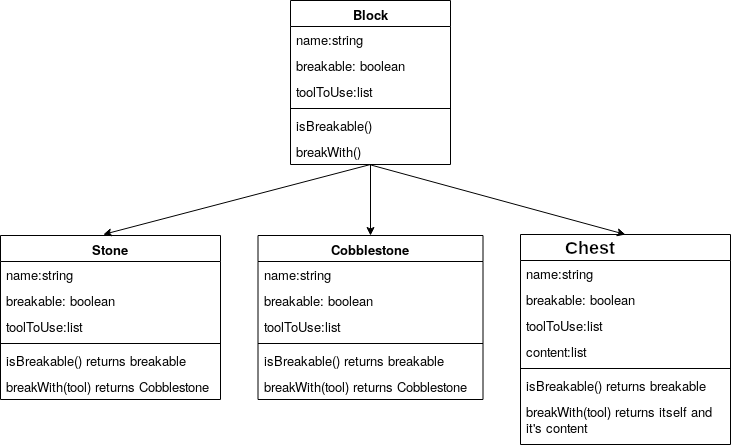
\includegraphics{Exercise8.png}
\caption{Schema}
\end{figure}

    \hypertarget{encapsulation}{%
\section{Encapsulation}\label{encapsulation}}

When programmin using classes we sometimes want to avoid the final user
to execute some method or access some attributes to avoid possible
mistakes and problems. We can doing this using encapsulation. Let's make
and example considering the class ``\emph{Student}'' defined below

    \begin{tcolorbox}[breakable, size=fbox, boxrule=1pt, pad at break*=1mm,colback=cellbackground, colframe=cellborder]
\prompt{In}{incolor}{40}{\boxspacing}
\begin{Verbatim}[commandchars=\\\{\}]
\PY{k}{class} \PY{n+nc}{Student}\PY{p}{(}\PY{n+nb}{object}\PY{p}{)}\PY{p}{:}
    \PY{k}{def} \PY{n+nf}{\PYZus{}\PYZus{}init\PYZus{}\PYZus{}}\PY{p}{(}\PY{n+nb+bp}{self}\PY{p}{,}\PY{n}{name}\PY{p}{,}\PY{n}{surname}\PY{p}{,}\PY{n}{birthday}\PY{p}{)}\PY{p}{:}
        \PY{n+nb+bp}{self}\PY{o}{.}\PY{n}{name}\PY{o}{=}\PY{n}{name}
        \PY{n+nb+bp}{self}\PY{o}{.}\PY{n}{surname}\PY{o}{=}\PY{n}{surname}
        \PY{n+nb+bp}{self}\PY{o}{.}\PY{n}{birthday}\PY{o}{=}\PY{n}{birthday}
\PY{k}{if} \PY{n+nv+vm}{\PYZus{}\PYZus{}name\PYZus{}\PYZus{}}\PY{o}{==}\PY{l+s+s2}{\PYZdq{}}\PY{l+s+s2}{\PYZus{}\PYZus{}main\PYZus{}\PYZus{}}\PY{l+s+s2}{\PYZdq{}}\PY{p}{:}
    \PY{c+c1}{\PYZsh{}Create a student}
    \PY{n}{s}\PY{o}{=}\PY{n}{Student}\PY{p}{(}\PY{l+s+s2}{\PYZdq{}}\PY{l+s+s2}{Mickey}\PY{l+s+s2}{\PYZdq{}}\PY{p}{,}\PY{l+s+s2}{\PYZdq{}}\PY{l+s+s2}{Mouse}\PY{l+s+s2}{\PYZdq{}}\PY{p}{,}\PY{l+s+s2}{\PYZdq{}}\PY{l+s+s2}{16/01/1928}\PY{l+s+s2}{\PYZdq{}}\PY{p}{)}
    \PY{c+c1}{\PYZsh{}Print his full name}
    \PY{n+nb}{print}\PY{p}{(}\PY{n}{s}\PY{o}{.}\PY{n}{name}\PY{o}{+}\PY{l+s+s2}{\PYZdq{}}\PY{l+s+s2}{ }\PY{l+s+s2}{\PYZdq{}}\PY{o}{+}\PY{n}{s}\PY{o}{.}\PY{n}{surname}\PY{p}{)}
    \PY{c+c1}{\PYZsh{}Change the student\PYZsq{}s surname and print it again}
    \PY{n}{s}\PY{o}{.}\PY{n}{surname}\PY{o}{=}\PY{l+s+s2}{\PYZdq{}}\PY{l+s+s2}{Duck}\PY{l+s+s2}{\PYZdq{}}
    \PY{n+nb}{print}\PY{p}{(}\PY{n}{s}\PY{o}{.}\PY{n}{name}\PY{o}{+}\PY{l+s+s2}{\PYZdq{}}\PY{l+s+s2}{ }\PY{l+s+s2}{\PYZdq{}}\PY{o}{+}\PY{n}{s}\PY{o}{.}\PY{n}{surname}\PY{p}{)}
\end{Verbatim}
\end{tcolorbox}

    \begin{Verbatim}[commandchars=\\\{\}]
Mickey Mouse
Mickey Duck
    \end{Verbatim}

    As you see we can access to the attributes of the class without any
restriction. If we want instead to restrict the access to the attribute
\emph{name} and \emph{surname} to avoid the possibility to modify these
after the object creation, the attribute birthday instead well have the
same behaviour. To achieve this we would do as follows

    \begin{tcolorbox}[breakable, size=fbox, boxrule=1pt, pad at break*=1mm,colback=cellbackground, colframe=cellborder]
\prompt{In}{incolor}{41}{\boxspacing}
\begin{Verbatim}[commandchars=\\\{\}]
\PY{k}{class} \PY{n+nc}{Student}\PY{p}{(}\PY{n+nb}{object}\PY{p}{)}\PY{p}{:}
    \PY{k}{def} \PY{n+nf}{\PYZus{}\PYZus{}init\PYZus{}\PYZus{}}\PY{p}{(}\PY{n+nb+bp}{self}\PY{p}{,}\PY{n}{name}\PY{p}{,}\PY{n}{surname}\PY{p}{,}\PY{n}{birthday}\PY{p}{)}\PY{p}{:}
        \PY{n+nb+bp}{self}\PY{o}{.}\PY{n}{\PYZus{}\PYZus{}name}\PY{o}{=}\PY{n}{name}
        \PY{n+nb+bp}{self}\PY{o}{.}\PY{n}{\PYZus{}\PYZus{}surname}\PY{o}{=}\PY{n}{surname}
        \PY{n+nb+bp}{self}\PY{o}{.}\PY{n}{birthday}\PY{o}{=}\PY{n}{birthday}
    \PY{k}{def} \PY{n+nf}{getFullName}\PY{p}{(}\PY{n+nb+bp}{self}\PY{p}{)}\PY{p}{:}
        \PY{k}{return} \PY{n+nb+bp}{self}\PY{o}{.}\PY{n}{\PYZus{}\PYZus{}name}\PY{o}{+}\PY{l+s+s2}{\PYZdq{}}\PY{l+s+s2}{ }\PY{l+s+s2}{\PYZdq{}}\PY{o}{+}\PY{n+nb+bp}{self}\PY{o}{.}\PY{n}{\PYZus{}\PYZus{}surname}
\end{Verbatim}
\end{tcolorbox}

    If in this case we try to access the attributes \emph{\_\_name} or
\emph{\_\_surname} we would get an error. The only way to obtain the
complete name would be to use the method \emph{getFullName()}. So to use
encapsulation in Python and hide some attributes to the final user we
must simpply put ``\_\_'' before the name its name (the same can be done
to hide methods)

    \hypertarget{exercise-9}{%
\section{Exercise 9}\label{exercise-9}}

As exercise to exploit encapsulation let's create a class
``\emph{Car}'', the class must have the attributtes for name, speed and
gear with the following properties

\begin{enumerate}
\def\labelenumi{\arabic{enumi}.}
\tightlist
\item
  the \emph{name} can't be changed after the creation of the object, but
  it can be retrieved
\item
  the \emph{speed} can be set to any value less than 250 (if greater it
  will be changed to 250) and can be retrieved
\item
  the \emph{gear} can go from 1 to 6 and can be changed only up and down
  by one (it's set to 1 when the object is created) and can be retrieved
\end{enumerate}

    \begin{tcolorbox}[breakable, size=fbox, boxrule=1pt, pad at break*=1mm,colback=cellbackground, colframe=cellborder]
\prompt{In}{incolor}{ }{\boxspacing}
\begin{Verbatim}[commandchars=\\\{\}]

\end{Verbatim}
\end{tcolorbox}


    % Add a bibliography block to the postdoc
    
    
    
\end{document}
